\chapter[SCP-172 齿轮人]{
    SCP-172 The Gearman\\
    SCP-172 齿轮人
}

\label{chap:SCP-172}

\begin{figure}[H]
    \centering
    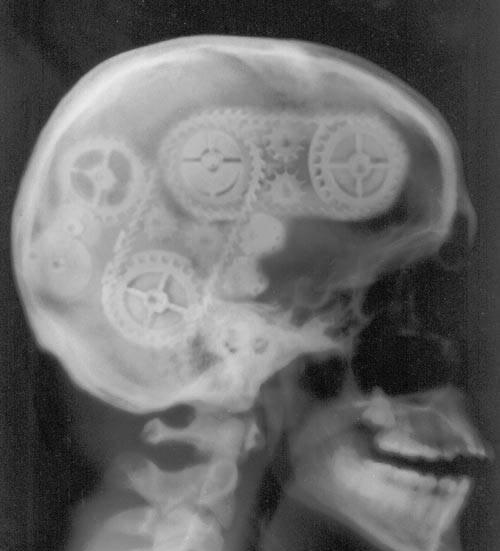
\includegraphics[width=0.5\linewidth]{images/SCP-172.jpg}
    \caption*{SCP-172的初始X光照片}
\end{figure}

\bb{项目编号:}SCP-172

\bb{项目等级:}Euclid

\bb{特殊收容措施:}任何希望接触SCP-172的人员必须进行书面申请,并进行一个小时的训练课程。任何与SCP-172的互动必须处于至少一名4级人员的监视下,且该人员有权根据自己的判断终止互动。所有由SCP-172提供的记录,图纸,书信必须马上提交给█████博士检查。任何由SCP-172提出的合理要求可以在█████博士批准后予以满足。SCP-172可以在经过批准后离开收容区域,不过全程必须有一名4级武装密探陪同。

武装人员将在SCP-172的门外执勤。若SCP-172试图逃脱,应主要通过口头要求其停止其举动,并将其带回收容区域。收容区域应该储存纸张,铅笔,以及SCP-172要求的任何附加组件。桌子,椅子,以及SCP-172要求的其他家具可以在经█████博士批准后予以提供。若进入休眠状态,SCP-172应放置在它的运输盒内直到其恢复。

\bb{描述:}SCP-172是一名34岁的人类,身高185厘米(6英寸1英尺)。,黑色的头发和胡子,体重175.5公斤(386磅),俄国血统。SCP-172的个性是友好和睿智的,虽然有点呆板。SCP-172偏好1860年代的服饰,并一直在脖子上佩戴一根连着一把华丽的大钥匙的长项链。SCP-172从没有透露其姓名,且被用指定号码称呼时并没有生气。

SCP-172的内部则是各种出奇复杂的自动机构,拥有200万个可动部件,并根据上次的检查结果有800万个组件。组件的构成是玻璃,丝绸,木头,钢铁,黄铜,橡胶以及其他多种物质。此种构造与\hyperref[chap:SCP-2776]{SCP-2776}的构造的相似表明俩者间有相似的创造者(们)。SCP-172同时还有数个可以从其胸口的舱口装入的“模块”。其体腔内各个位置的组件似乎决定了其行为,语言,运动等其他参数。SCP-172当前有46个模块,其中三个是在基金会的监管下制造的。当前,SCP-172装载了“工程师”组件。这些组件被SCP-172称之为“看守”,“士兵”,“医生”,“母亲”和“国王”,虽然这绝对不是全部的组件清单(参阅文件\#172-2)。任何情况下不经过O5级批准不得重置模块。

SCP-172的主要动力,是由其自己保管的钥匙,通过将钥匙插入其脖子底部的一个洞内来启动。简单的上一次“发条”可以让SCP-172运转8个小时。SCP-172在启动时和普通人类几乎没有不同,并具有所有基础的人类功能。SCP-172不需要进食,呼吸,或睡眠,但是在可能的情况其会和普通人类一样进行这些行为。SCP-172十分合作,并对任何给予其的指令尽量做到最好。

SCP-172并不觉得自己的存在是奇怪的,即使在其内部组件暴露在外的情况下也声称自己是人类。SCP-172同时也是十分脆弱的,必须十分注意保护以维护其功能。SCP-172同时表现出奇迹一般的机械技术水平。SCP-172可以分析和复制任何其所接触到的机械设备。这个天赋第一次被发现是因为基金会人员发现几乎任何锁都无法锁住SCP-172。其同时还根据基金会的科技制作了数个复制品甚至是“升级”品,全部这些产品的运作都是基于极为复杂的发条机构。特别要注意的是,{[}数据删除]。

\hr

\bb{文件\#172-4R:}SCP-172的回收备忘录

SCP-172回收于第一次世界大战结束后,一个曾经是沙皇的别墅的地下室内。该地下室因为流弹轰炸而被暴露出来,地下室及其内部都严重受损,不过SCP-172被发现完好无损的保存在一个铁箱内,包括许多“模块”和它的钥匙。这些物品被密探回收,并在测试设施内进行“恢复”。SCP-172似乎是从一次深层睡眠中醒来,并用俄语对面前的每个人打招呼。当████████████特工还处于震惊中时,SCP-172推了一下自己的胸,并重新用英语打了个招呼。SCP-172在问讯中,表示其最后的记忆是在和一个小男孩玩。当男孩离开后,它觉得“很累”,于是返回盒子内。它没有关于其制造过程,制造者,以及名字的记忆。
